%%%%%%%%%%%%%%%%%%%%%%%%%%%%%%%%%%%%%%%%%
% University Assignment Title Page 
% LaTeX Template
% Version 1.0 (27/12/12)
%
% This template has been downloaded from:
% http://www.LaTeXTemplates.com
%
% Original author:
% WikiBooks (http://en.wikibooks.org/wiki/LaTeX/Title_Creation)
%
% License:
% CC BY-NC-SA 3.0 (http://creativecommons.org/licenses/by-nc-sa/3.0/)
% 
% Instructions for using this template:
% This title page is capable of being compiled as is. This is not useful for 
% including it in another document. To do this, you have two options: 
%
% 1) Copy/paste everything between \begin{document} and \end{document} 
% starting at \begin{titlepage} and paste this into another LaTeX file where you 
% want your title page.
% OR
% 2) Remove everything outside the \begin{titlepage} and \end{titlepage} and 
% move this file to the same directory as the LaTeX file you wish to add it to. 
% Then add \input{./title_page_1.tex} to your LaTeX file where you want your
% title page.
%
%%%%%%%%%%%%%%%%%%%%%%%%%%%%%%%%%%%%%%%%%
%\title{Title page with logo}
%----------------------------------------------------------------------------------------
%	PACKAGES AND OTHER DOCUMENT CONFIGURATIONS
%----------------------------------------------------------------------------------------

\documentclass[12pt]{article}
\usepackage[english]{babel}
\usepackage[utf8x]{inputenc}
\usepackage{amsmath}
\usepackage{graphicx}
\usepackage[colorinlistoftodos]{todonotes}
\usepackage{hyperref}

\begin{document}

\begin{titlepage}

\newcommand{\HRule}{\rule{\linewidth}{0.5mm}} % Defines a new command for the horizontal lines, change thickness here

\center % Center everything on the page
 
%----------------------------------------------------------------------------------------
%	HEADING SECTIONS
%----------------------------------------------------------------------------------------

\textsc{\LARGE Università degli studi di Milano-Bicocca}\\[1cm] % Name of your university/college
\textsc{\Large Advanced Machine Learning }\\[0.3cm] % Major heading such as course name
\textsc{\large Final Project}\\[0.1cm] % Minor heading such as course title

%----------------------------------------------------------------------------------------
%	TITLE SECTION
%----------------------------------------------------------------------------------------

\HRule \\[0.4cm]
{ \huge \bfseries Floranet}\\[0.4cm] % Title of your document
\HRule \\[1.5cm]
 
%----------------------------------------------------------------------------------------
%	AUTHOR SECTION
%----------------------------------------------------------------------------------------

\large
\emph{Authors:}\\
Andrea Moleri - 902011 - a.moleri@campus.unimib.it \\   % Your name
Filippo Armani - 865939 - f.armani1@campus.unimib.it   \\[1cm] % Your name

% If you don't want a supervisor, uncomment the two lines below and remove the section above
%\Large \emph{Author:}\\
%John \textsc{Smith}\\[3cm] % Your name

%----------------------------------------------------------------------------------------
%	DATE SECTION
%----------------------------------------------------------------------------------------

{\large \today}\\[2cm] % Date, change the \today to a set date if you want to be precise

%----------------------------------------------------------------------------------------
%	LOGO SECTION
%----------------------------------------------------------------------------------------


\includegraphics{Images/logo}\\[1cm] % Include a department/university logo - this will require the graphicx package
 
%----------------------------------------------------------------------------------------

\vfill % Fill the rest of the page with whitespace

\end{titlepage}


\begin{abstract}
This report presents Floranet, a deep learning-based approach aimed at developing models capable of correctly
identifying flower species from images while minimizing classification errors. The investigation focused on leveraging
transfer learning techniques with three base architectures: VGG16, DenseNet121, and InceptionV3. Various methodologies,
including full and partial freezing of network layers and the application of data augmentation were tested to evaluate
their impact on model performance. The result is a suite of models capable of solving the classification problem with
high test accuracy and low error propensity.

\end{abstract}

\section{Introduction}
The classification of images has become a cornerstone task in the field of machine learning and deep learning due to
its wide range of applications, from medical diagnostics to automated systems in agriculture. This project, titled
Floranet, focuses on the classification of flower species using the \href{https://www.robots.ox.ac.uk/~vgg/data/flowers/102/index.html}{Oxford Flower Dataset},
a dataset curated by Maria-Elena Nilsback and Andrew Zisserman. The dataset comprises 102 flower species, with the
number of images per species ranging from 40 to 258. These images present significant challenges due to variations in
scale, pose, lighting conditions, and intra-class diversity, as well as inter-class similarity.

The problem addressed by this project is the accurate classification of flower images into their respective species,
a task that requires robust models capable of handling the inherent complexity of the dataset. To tackle this problem,
transfer learning was used, a technique that leverages pre-trained deep learning models to improve the efficiency and
accuracy of new tasks. Specifically, three state-of-the-art architectures were utilized. The aim was to investigate the
strengths and limitations of each one, offering insights into the performance of different architectures when applied
to complex classification tasks. The subsequent sections will delve into the detailed methodology, experimental
results, and an analysis of the findings.

\section{Datasets}
The dataset used in this project is the \href{https://www.robots.ox.ac.uk/~vgg/data/flowers/102/index.html}{Oxford Flower Dataset},
introduced in 2008 by Maria-Elena Nilsback and Andrew Zisserman. This dataset is designed for image classification tasks
and consists of 102 categories of flowers commonly found in the United Kingdom. The dataset includes three primary components:

\begin{itemize}
 \item \textbf{Image Files} (`102flowers.tgz`): high-resolution flower images across all 102 categories.
 \item \textbf{Segmentation Masks} (`102segmentations.tgz`): optional masks that define flower regions in the images (not utilized in this study).
 \item \textbf{Labels} (`imagelabels.mat`): class labels for each image, provided in MATLAB format.
\end{itemize}

To prepare the dataset, the required files were downloaded, decompressed, and organized into meaningful directories.
A Python script was implemented to automatically handle this process, ensuring that any missing files were downloaded
and verified. Class labels were extracted from the MATLAB file (`imagelabels.mat`) and adjusted for Python’s zero-based
indexing. To facilitate analysis, a mapping between class indices and their corresponding flower names was created using
the official dataset documentation. The image files were matched to their labels and organized into a structured Pandas
DataFrame, where each row contains the image file name and the associated flower name. While this step is not strictly
necessary for training machine learning models, it aids in exploratory data analysis and ensures that the dataset is
correctly understood and annotated. The dataset's original benchmark, as described in its publication, utilized
hand-crafted features for classification. This project, however, leverages CNN-based approaches, exploring the
advantages of transfer learning with pre-trained deep learning architectures.

The dataset poses significant challenges due to its inherent imbalance: the most populated class contains 258 images
(Petunia), while the least populated class includes only 40 images (e.g., Pink Primrose). A quantitative analysis
[Fig.1] reveals that the average number of images per class is 80.28, with substantial variance indicating the presence
of class imbalance. To address this issue, a data augmentation strategy was implemented to ensure a more uniform distribution
across classes. The augmentation included transformations such as rotation, width shift, height shift, zoom, and flips.

\begin{figure}[h!]
    \centering
    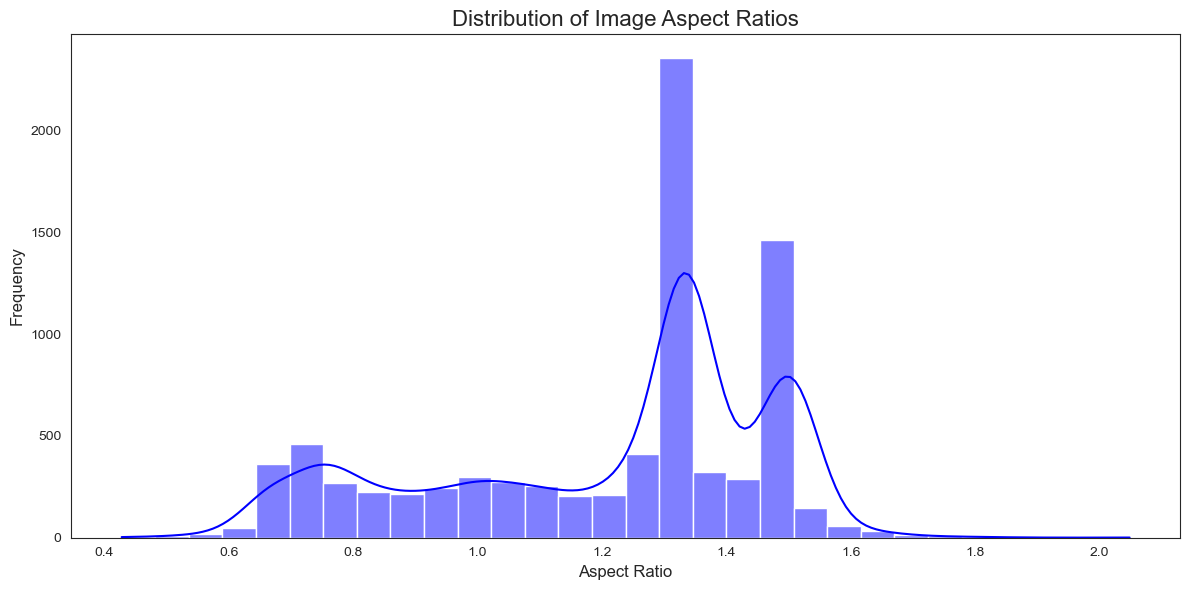
\includegraphics[width=\linewidth]{Images/Distribution of Image Aspect Ratios}
    \caption{Distribution of Image Aspect Ratios}
\end{figure}


Qualitative insights into the dataset were gained through visualizations. A bar plot [Fig.2] of class distributions highlights
the imbalance, while a subset of images from the top five most populated classes [Fig.3] showcases intra-class variability,
pose variations, and image quality. For instance, the Petunia class exhibits notable pose diversity, while inter-class
similarity is observed between Wallflower and Watercress. Additionally, intra-class variation is evident in the Water
Lily class, where samples within the same category differ significantly in appearance. Such variability may increase
the complexity of the classification task, necessitating robust feature extraction techniques.

\begin{figure}[h!]
    \centering
    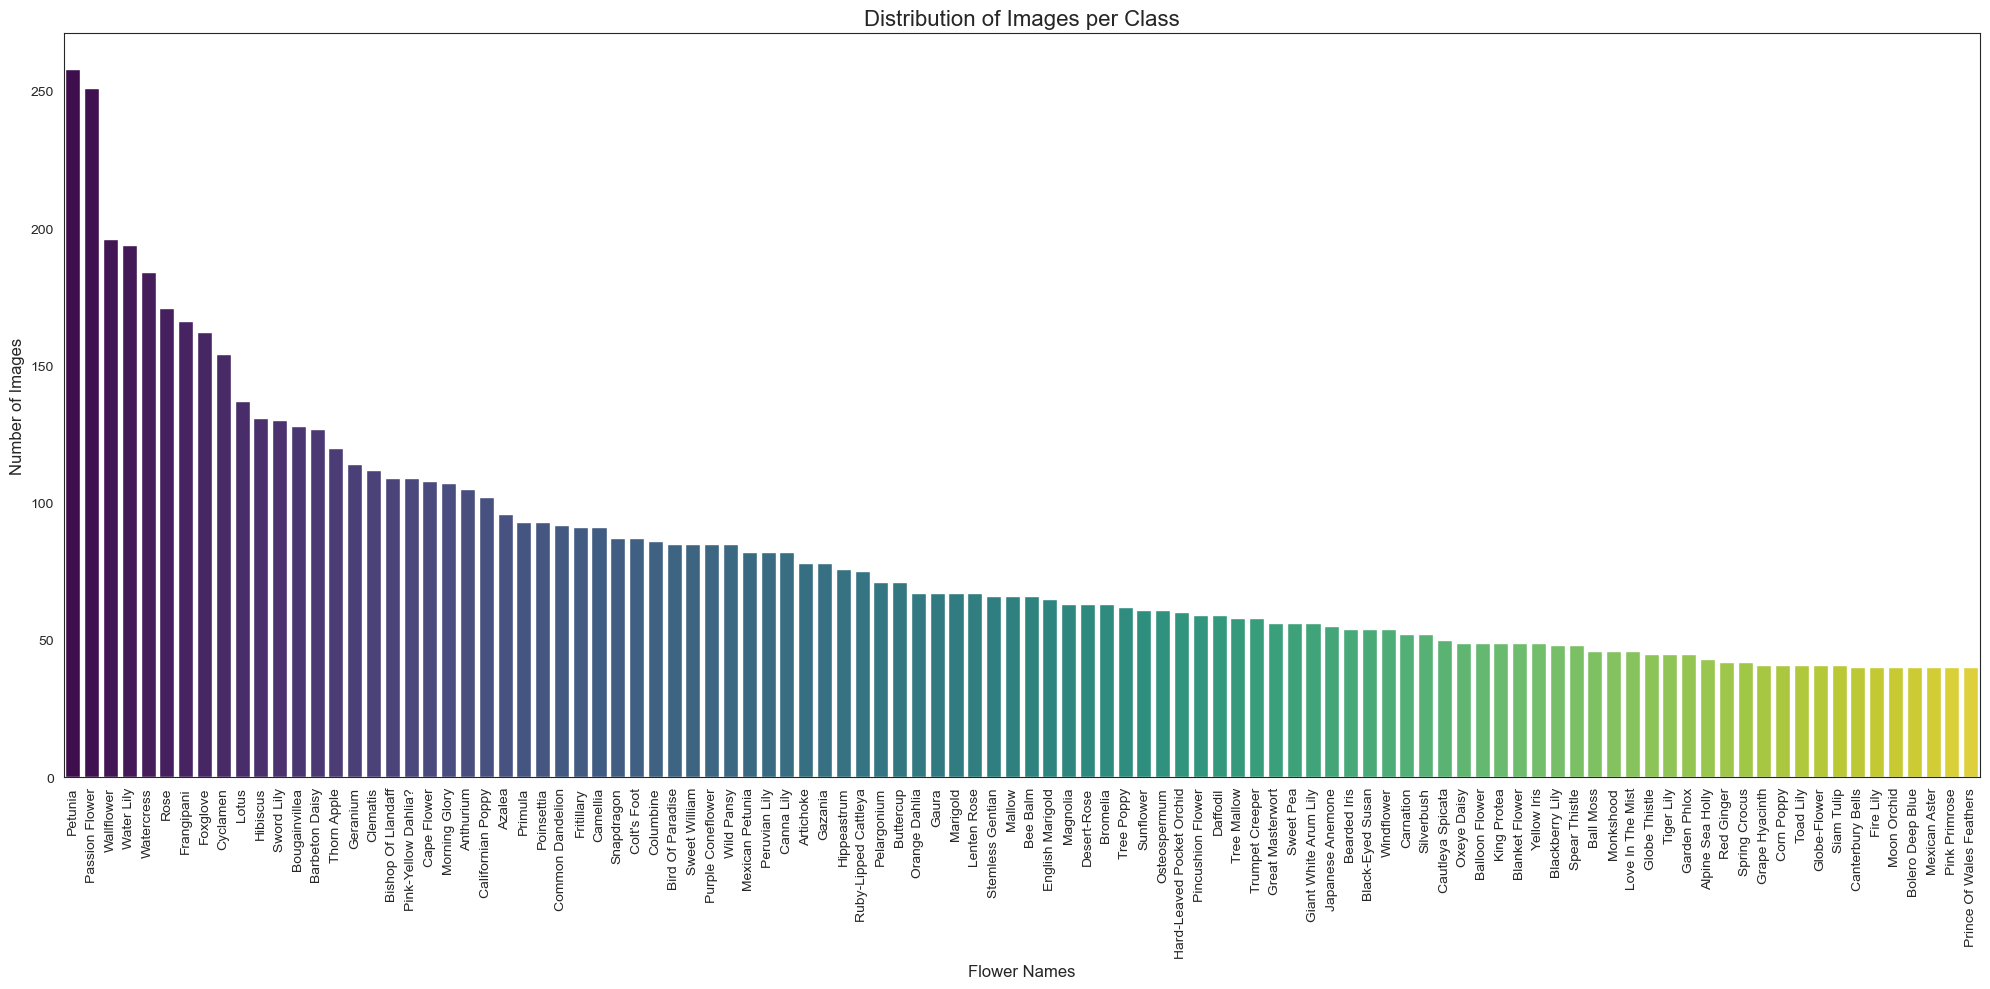
\includegraphics[width=\linewidth]{Images/Distribution of Images per Class}
    \caption{Distribution of Images per Class}
\end{figure}

\begin{figure}[h!]
    \centering
    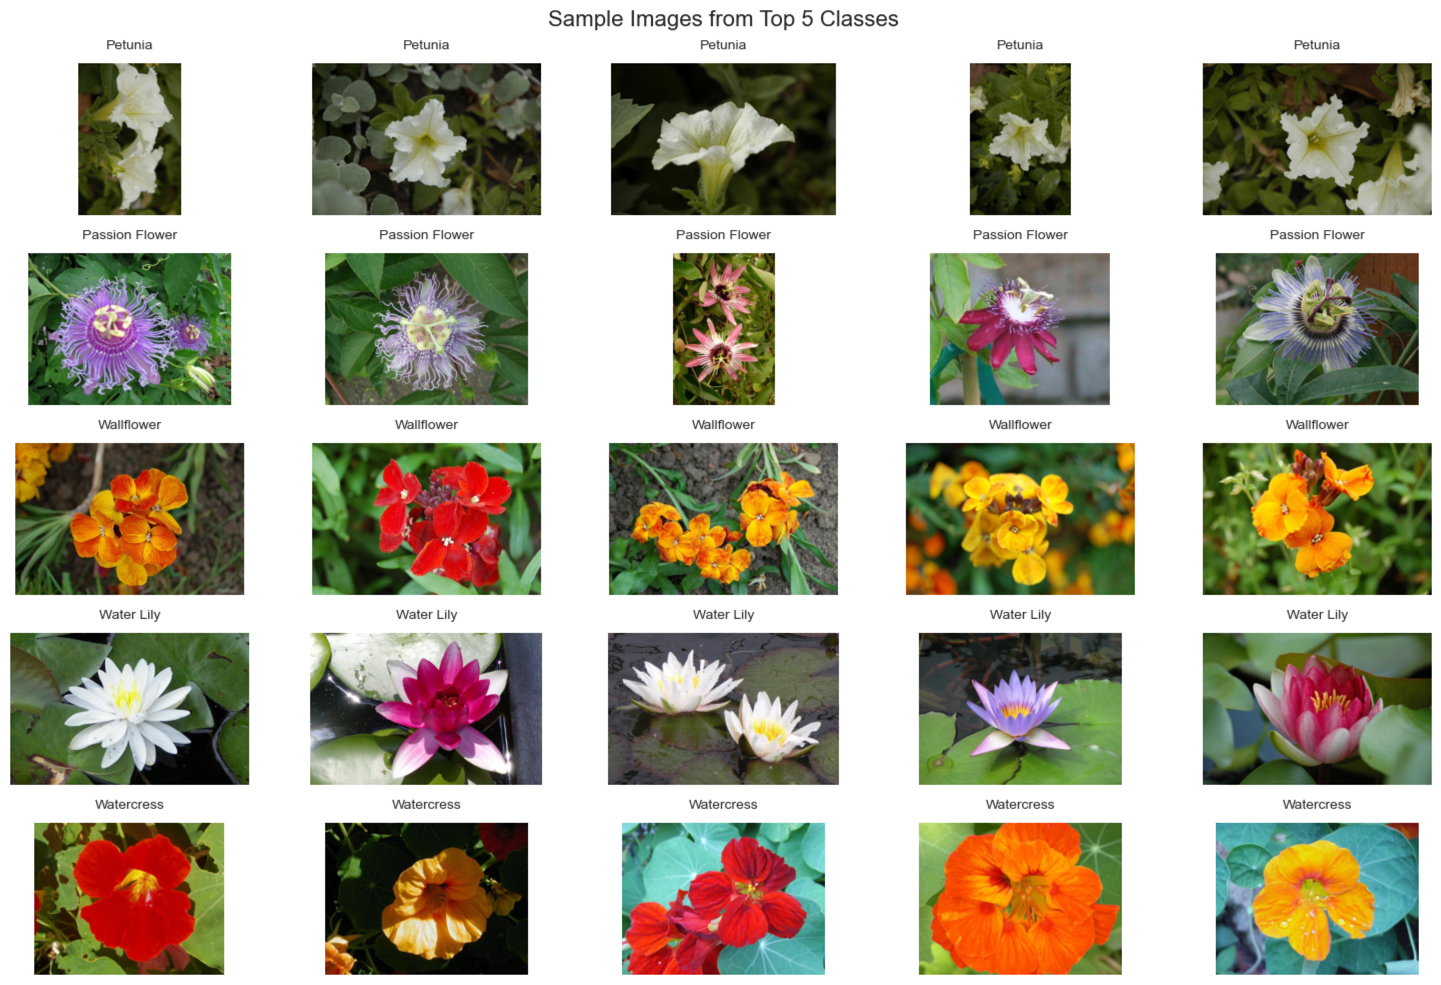
\includegraphics[width=\linewidth]{Images/Sample Images from Top 5 Classes}
    \caption{Sample Images from Top 5 Classes}
\end{figure}

To further understand the dataset's characteristics, the dimensions of all images were analyzed, yielding an average
resolution of approximately \(630 \times 534\) pixels. The aspect ratio distribution centers around 1.2, with minor
outliers. This uniformity in image dimensions simplifies preprocessing requirements but necessitates consistent
resizing for compatibility with convolutional neural networks. Furthermore, a comparison is made between flowers
extracted from 10 randomly selected classes, and flowers extracted from a specific class [Fig.4]. This visualization was made
to underscore the diversity within the dataset, and to highlight the consistency of samples for a particular category at the same time.

\begin{figure}[h!]
    \centering
    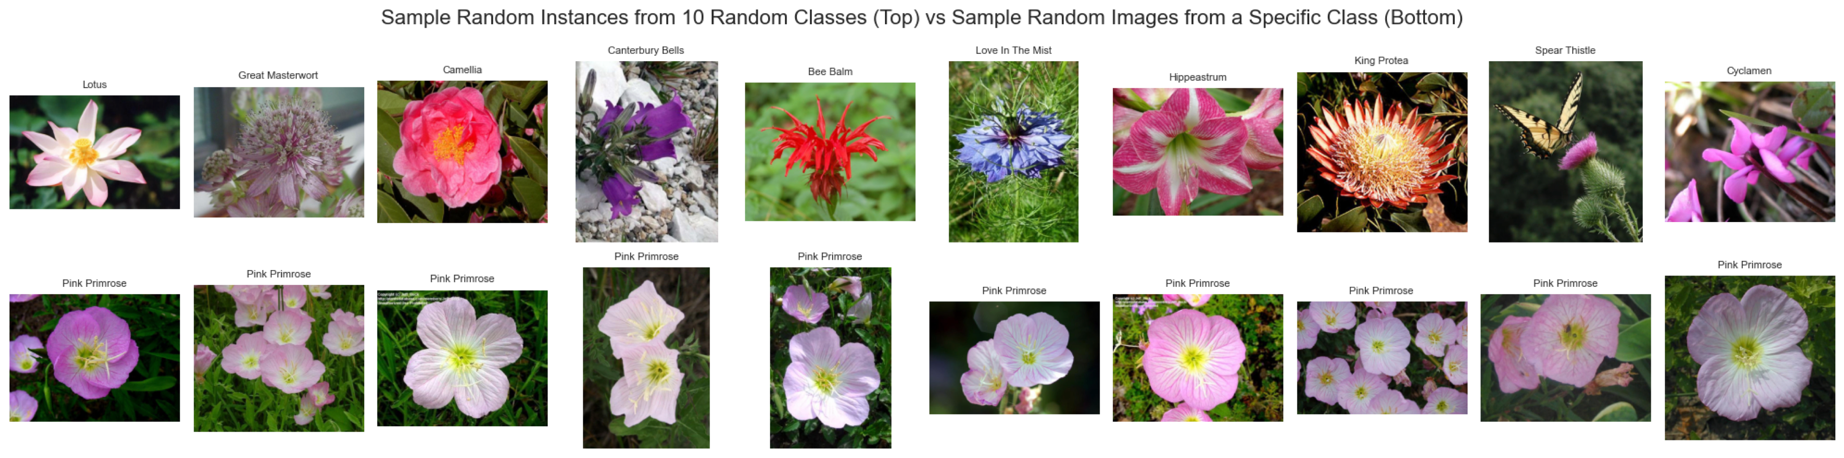
\includegraphics[width=\linewidth]{Images/Sample Random Instances from 10 Random Classes (Top) vs Sample Random Images from a Specific Class (Bottom)}
    \caption{Sample Images from Top 5 Classes}
\end{figure}


\section{The Methodological Approach}

This is the central and most important section of the report. Its objective must be to show, with linearity and clarity, the steps that have led to the definition of a decision model. The description of the working hypotheses, confirmed or denied, can be found in this section together with the description of the subsequent refining processes of the models. Comparisons between different models (e.g. heuristics vs. optimal models) in terms of quality of solutions, their explainability and execution times are welcome. 

Do not attempt to describe all the code in the system, and do not include large pieces of code in this section, use pseudo-code where necessary. Complete source code should be provided separately (in Appendixes, as separated material or as a link to an on-line repo). Instead pick out and describe just the pieces of code which, for example:
\begin{itemize}
\item are especially critical to the operation of the system;
\item you feel might be of particular interest to the reader for some reason;
\item  illustrate a non-standard or innovative way of implementing an algorithm, data
structure, etc..
\end{itemize}

You should also mention any unforeseen problems you encountered when implementing the
system and how and to what extent you overcame them. Common problems are:
 difficulties involving existing software.


\section{Results and Evaluation}
The Results section is dedicated to presenting the actual results (i.e. measured and calculated quantities), not to discussing their meaning or interpretation. The results should be summarized using appropriate Tables and Figures (graphs or schematics). Every Figure and Table should have a legend that describes concisely what is contained or shown. Figure legends go below the figure, table legends above the table. Throughout the report, but especially in this section, pay attention to reporting numbers with an appropriate number of significant figures. 

\section{Discussion}
The discussion section aims at interpreting the results in light of the project's objectives. The most important goal of this section is to interpret the results so that the reader is informed of the insight or answers that the results provide. This section should also present an evaluation of the particular approach taken by the group. For example: Based on the results, how could the experimental procedure be improved? What additional, future work may be warranted? What recommendations can be drawn?


\section{Conclusions}
Conclusions should summarize the central points made in the Discussion section, reinforcing for the reader the value and implications of the work. If the results were not definitive, specific future work that may be needed can be (briefly) described. The conclusions should never contain ``surprises''. Therefore, any conclusions should be based on observations and data already discussed. It is considered extremely bad form to introduce new data in the conclusions.

\section*{References}

The references section should contain complete citations following standard form.  The references should be numbered and listed in the order they were cited in the body of the report. In the text of the report, a particular reference can be cited by using a numerical number in brackets as \cite{Lee2015} that corresponds to its number in the reference list. \LaTeX provides several styles to format the references

\bibliographystyle{IEEEtran}
\bibliography{references.bib}

\end{document}